\section{Installazione}
\hypertarget{section::\theHsection}
Per l'esecuzione del software sviluppato è necessario aprire l'applicazione in locale tramite le istruzioni di seguito riportate.

\lstinputlisting[language=Bash]{Codice/run_from_terminal.bash}

\begin{figure}[h]
\centering
{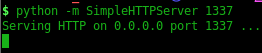
\includegraphics[scale=1]{Immagini/python_virtual_server.png}}
\caption{Virtual server in esecuzione}
\end{figure}

\newpage

Questa modalità di visualizzazione del sito presuppone che il sito sia già compilato per versione di produzione.

Se invece si volesse lanciare il sito dal codice sorgente, seguire le seguenti istruzioni.

\lstinputlisting[language=Bash]{Codice/run_from_terminal_versione_dev.bash}

\begin{figure}[h]
\centering
{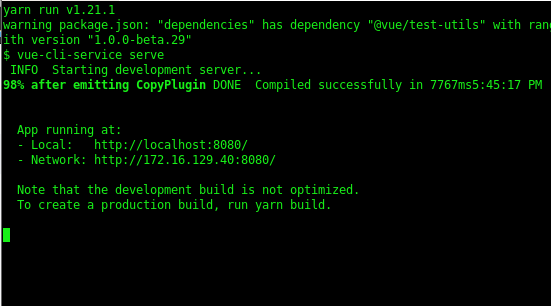
\includegraphics[scale=0.8]{Immagini/yarn_serve_localhost.png}}
\caption{"yarn serve" sito versione development in esecuzione}
\end{figure}

Il building si può fare con i seguenti commandi.

\lstinputlisting[language=Bash]{Codice/run_from_terminal_versione_build.bash}

\newpage

\begin{figure}[h]
\centering
{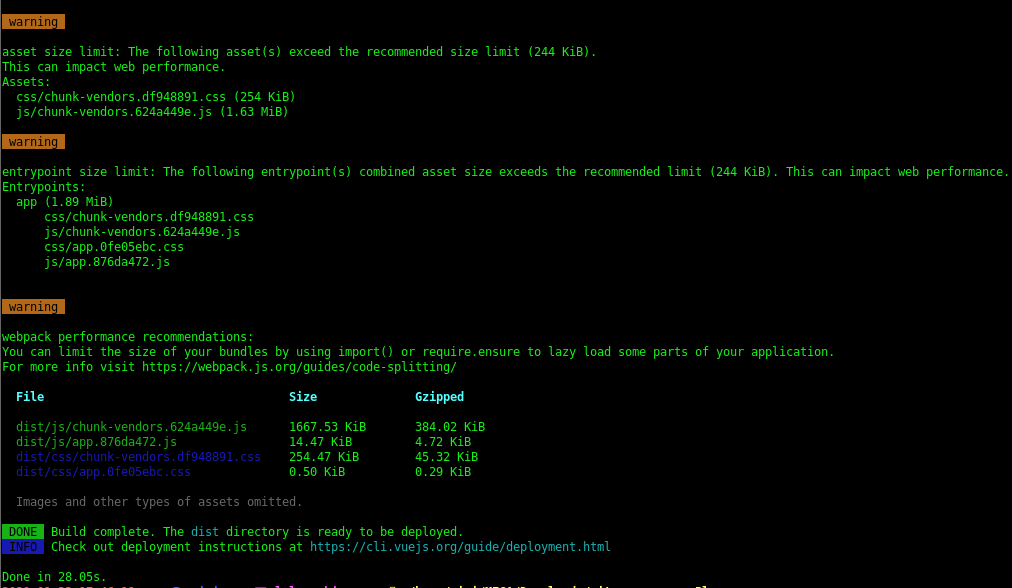
\includegraphics[scale=0.4]{Immagini/yarn_build_dist.png}}
\caption{"yarn build" compilazione del sito versione di produzione}
\end{figure}

\newpage

Una volta che le istruzioni sopra citate sono state eseguite verrà aperta una porta in locale nel proprio pc (ad.esempio http://localhost:8080/) con una schermata come riportato nella Figura 10.2. \autocite[\protect\label{Dayley2014}][]{Dayley2014}

Si procede aprendo un qualsiasi browser web e incollando l'indirizzo trovato nella barra di ricerca e premendo invio, il browser restituirà la Homepage della WebApp sviluppata.

\newpage

\section{Utilizzo}
\hypertarget{section::\theHsection}
In questa sezione verrà mostrato l'utilizzo dell'applicazione web sviluppata.
All'apertura della pagina web verrà mostrata una schermata contenente le caselle da riempire con i dati richiesti ed una mappa per la successiva visualizzazione.
Dopo l'inserimento dell'indirizzo sul proprio browser web verrà mostrato a schermo una pagina come nella Figura 10.4

La schermata è composta da 3 campi:
\begin{enumerate}
\item\textbf{Departure Address}: in questo campo deve essere inserita la città di partenza con l'eventuale indirizzo di partenza;
\item\textbf{Arrival Address}: in questo campo deve essere inserita la città di destinazione con l'eventuale indirizzo di destinazione;
\item\textbf{Car Autonomy}: in questo campo va inserita l'autonomia del proprio veicolo elettrico.
\end{enumerate}
\newpage
Il sistema è in grado di offrire dei suggerimenti riguardo l'inserimento delle destinazioni iniziali e finali e fare un check dei valori inseriti prima dell'invio al sistema.
In particolare nel campo autonomia non sono ammessi valori negativi ma soltanto valori compresi tra 1 e 1000 km.

\begin{figure}[h]
\centering
{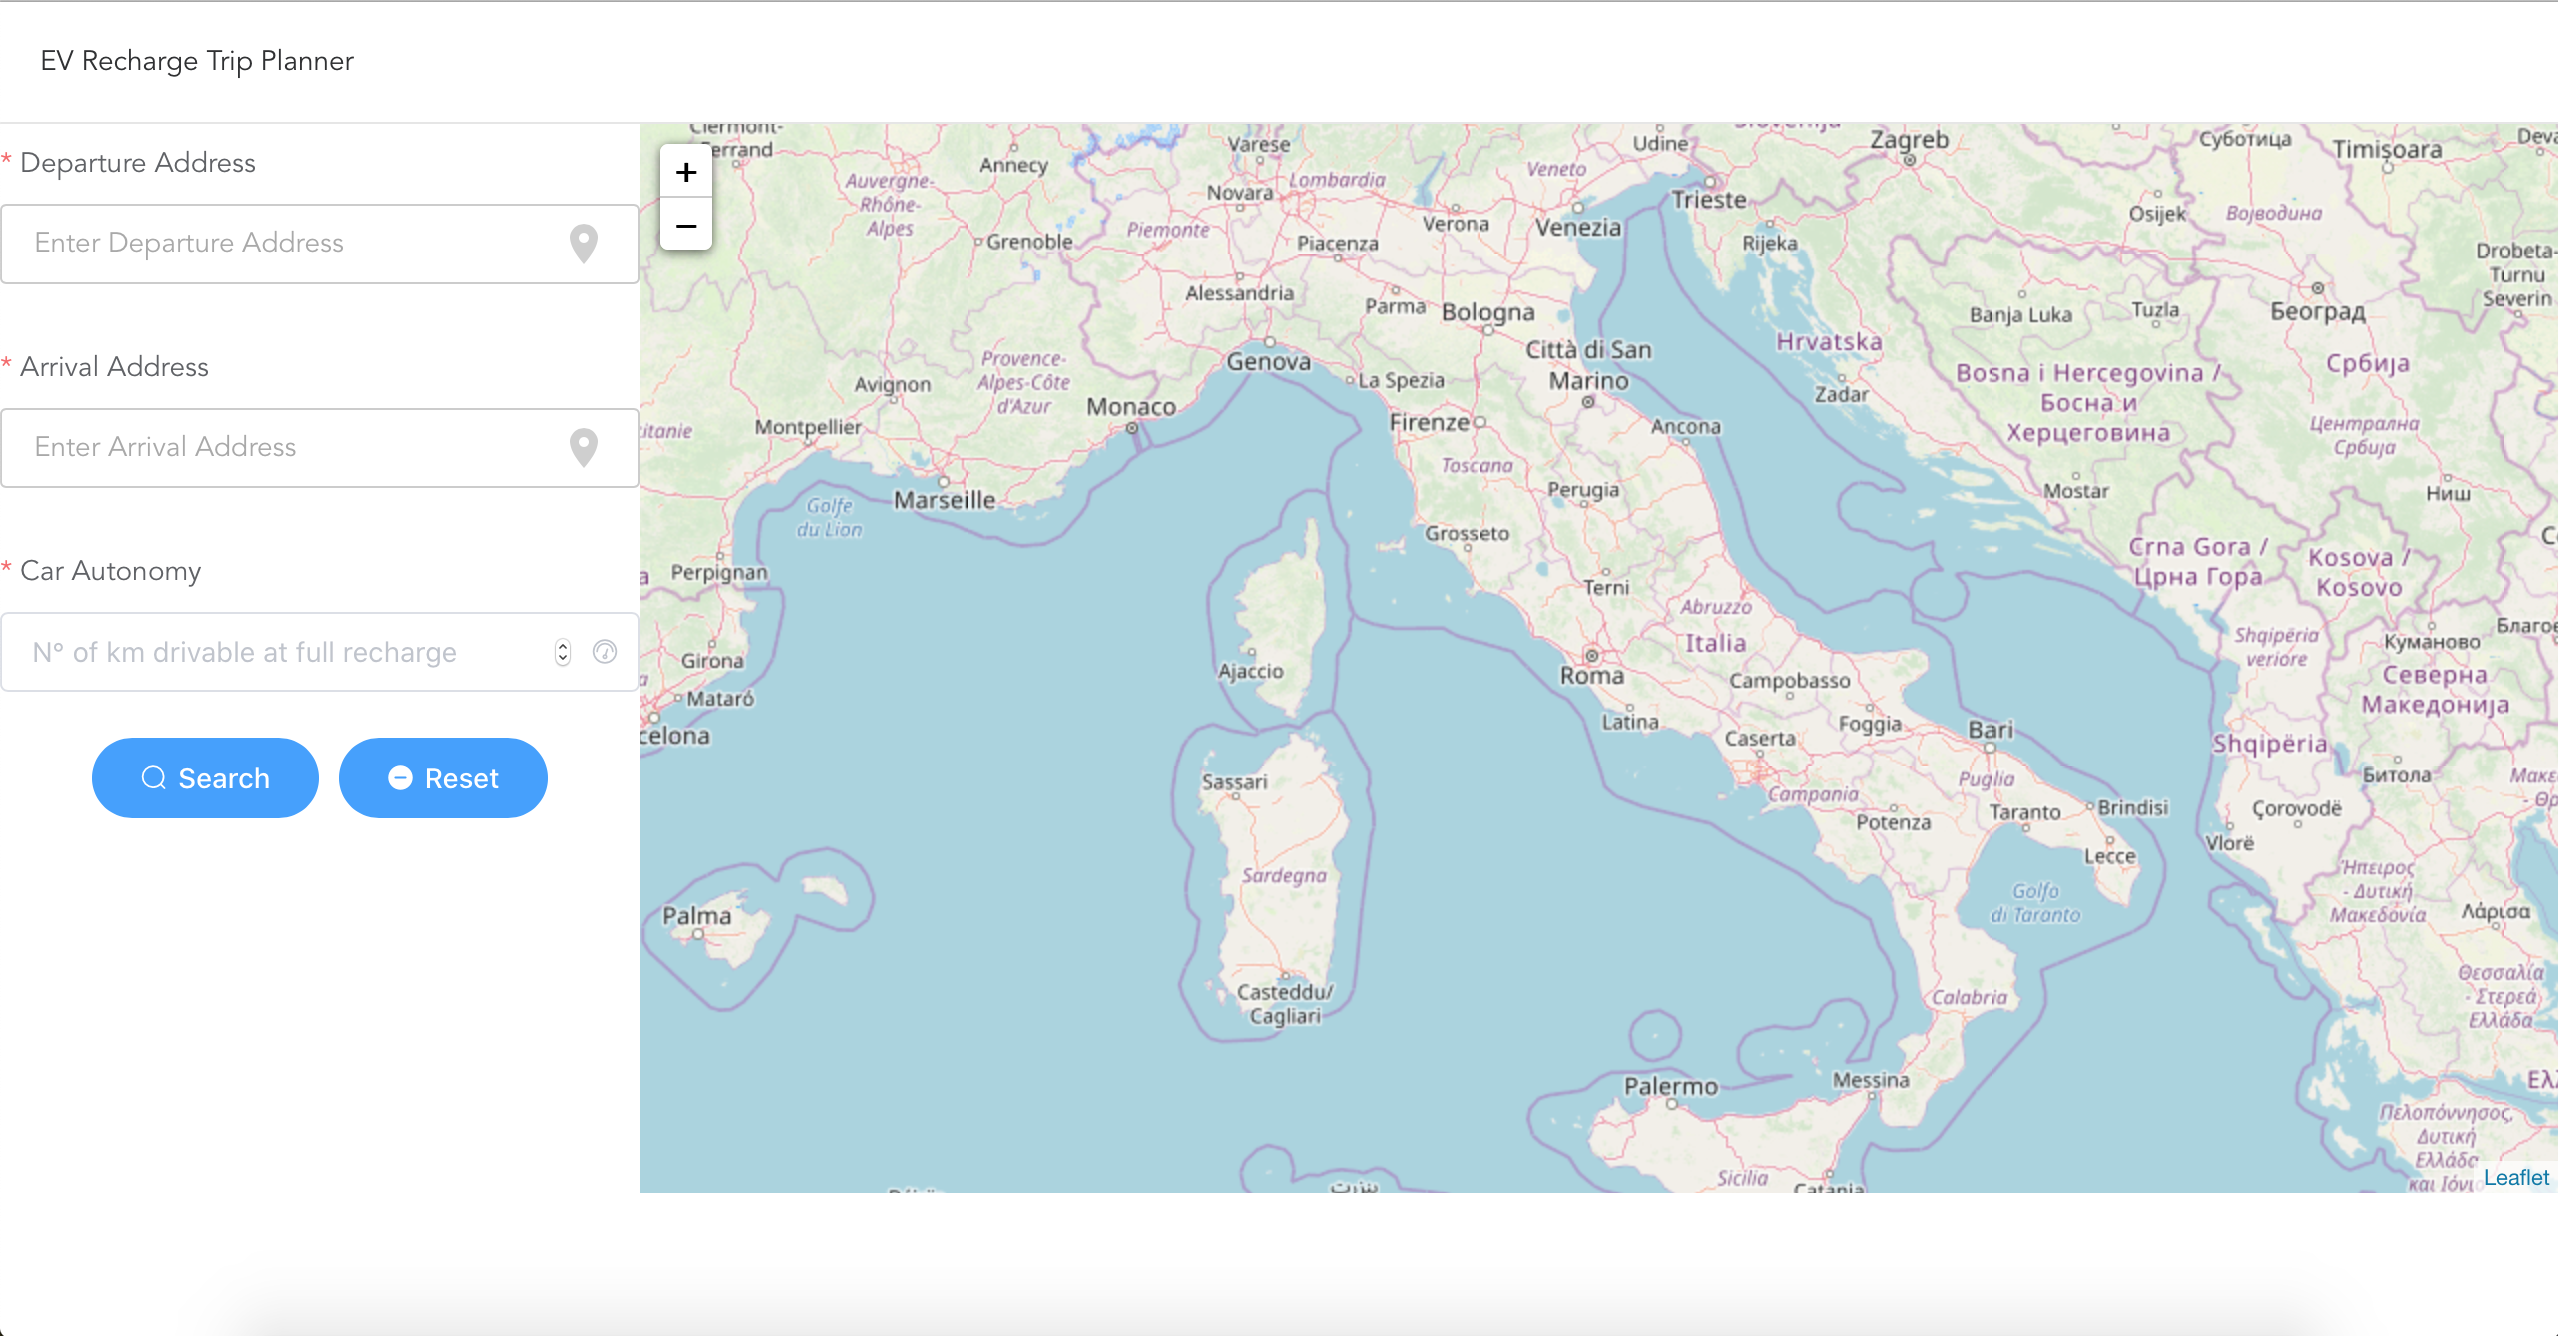
\includegraphics[scale=0.3]{Immagini/Schermata_Homepage.png}}
\caption{Schermata Homepage}
\end{figure}

Una volta inseriti nella schermata i dati 
richiesti, l'utente dovrà premere il pulsante Search come mostrato in Figura 10.5.

Il sistema risponderà con una schermata come in Figura 10.6 dove viene mostrato sulla mappa il punto iniziale e finale con il percorso da effettuare e le eventuali fermate.

\begin{figure}[h]
\centering
{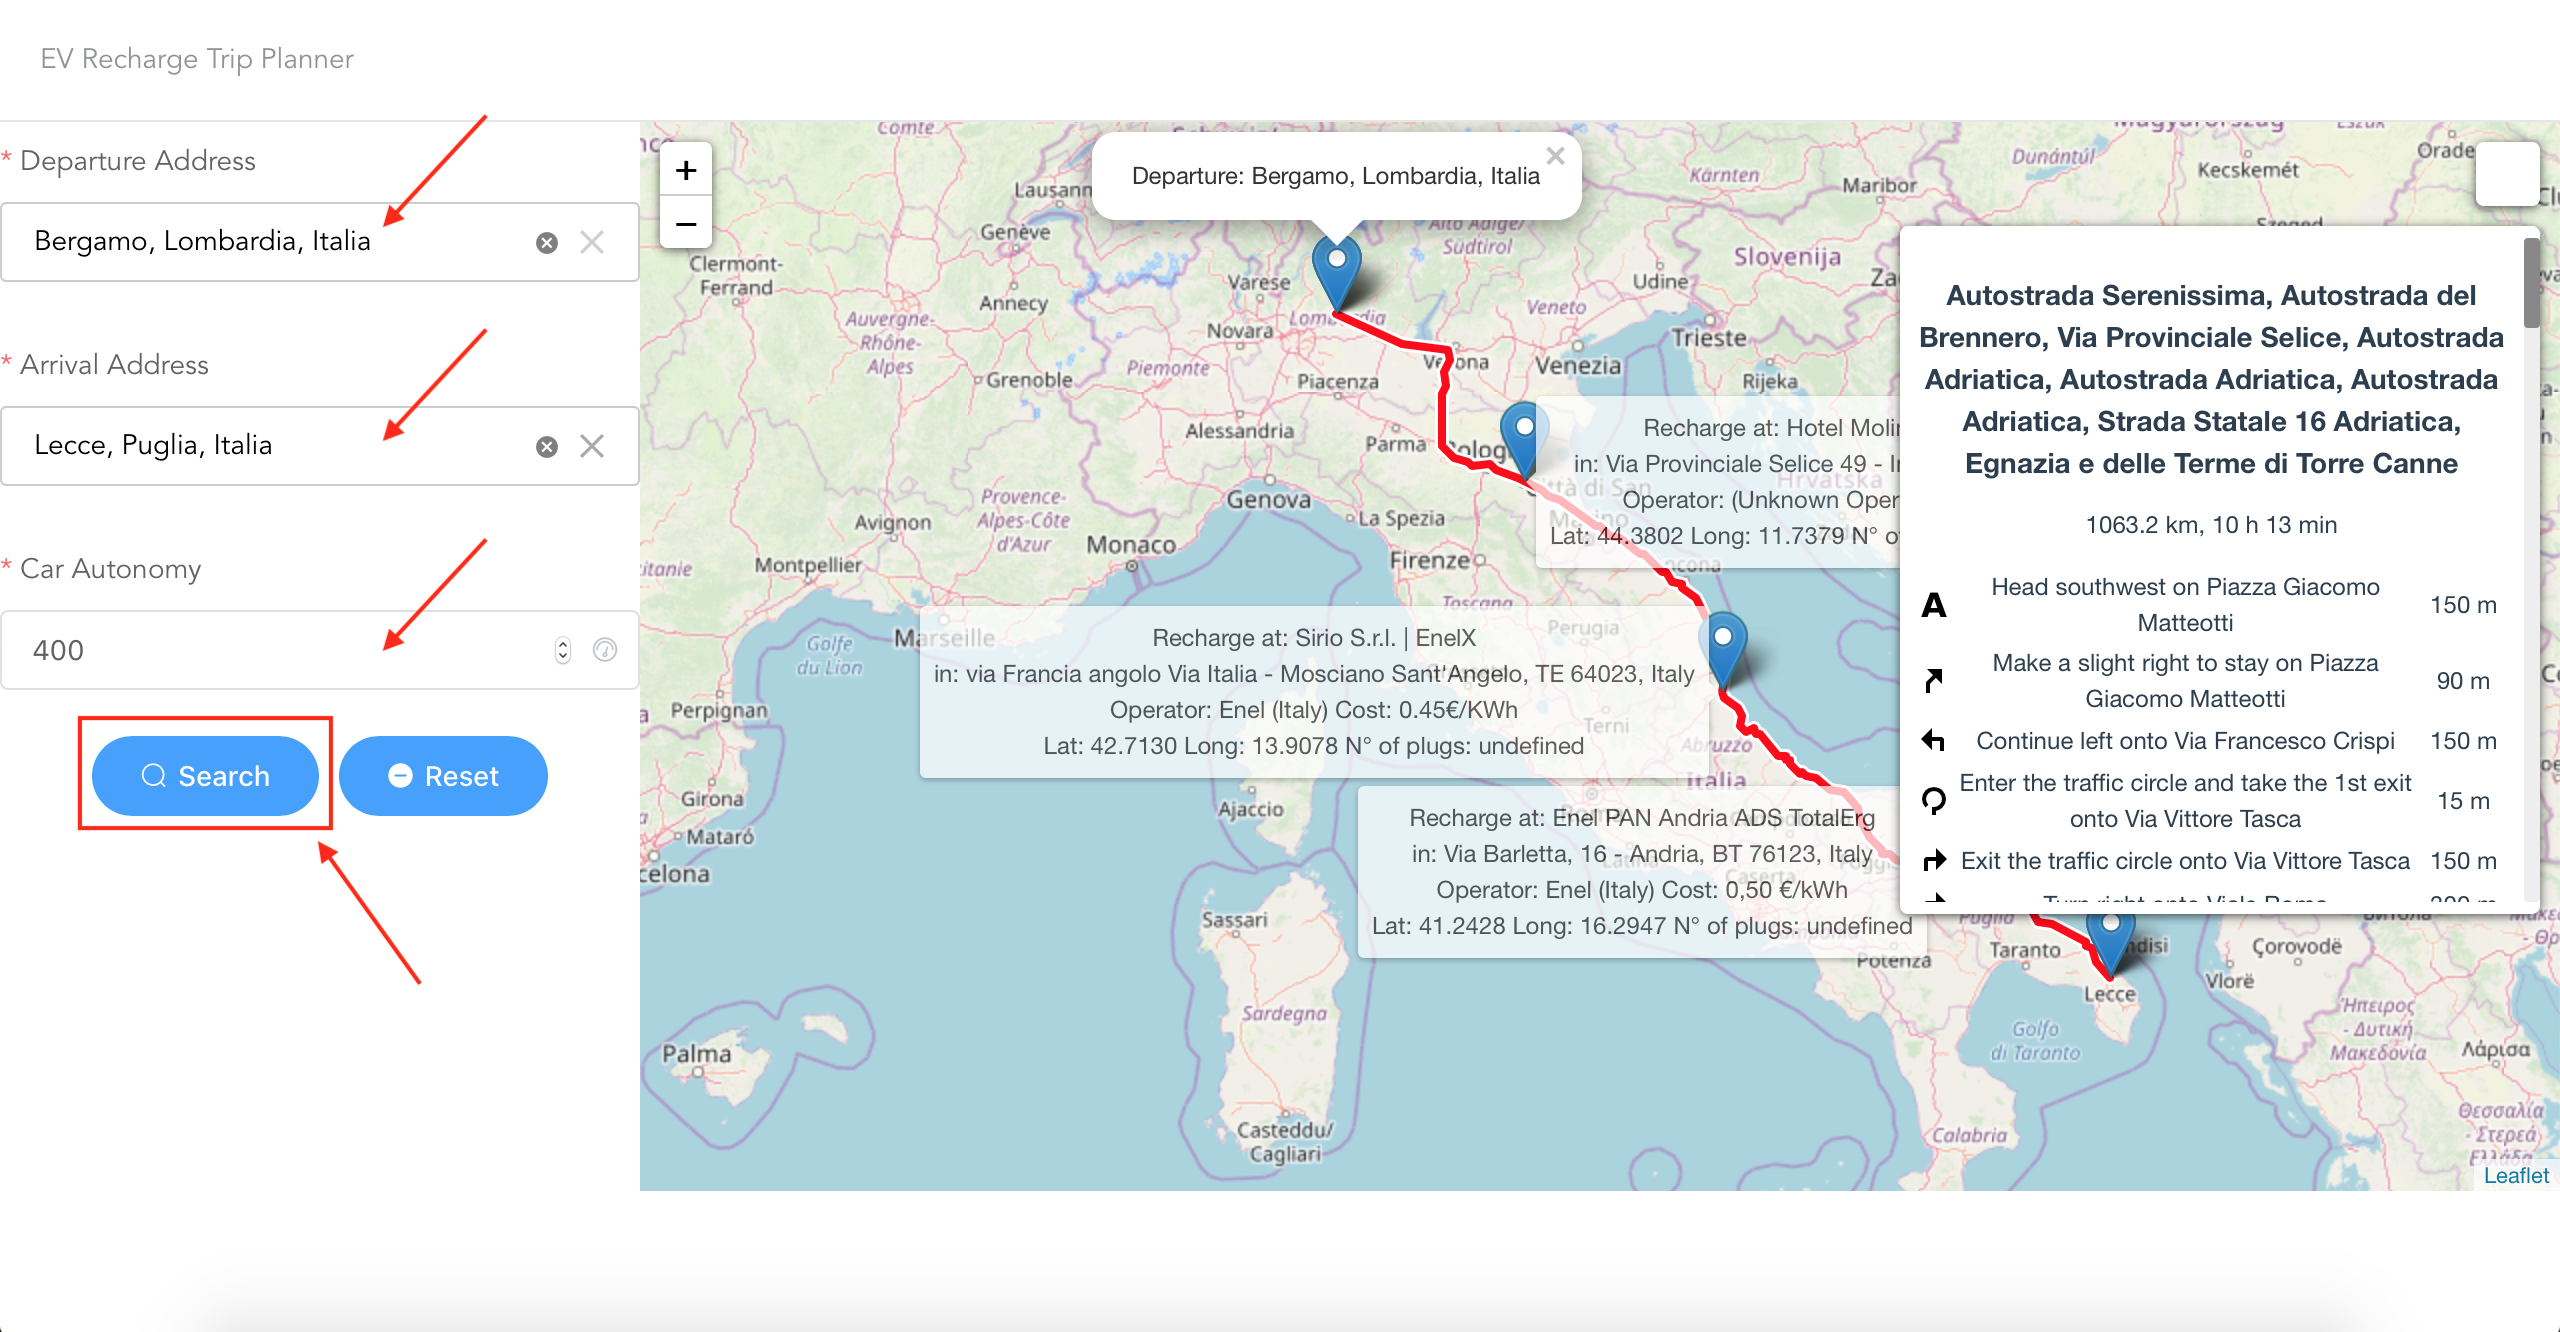
\includegraphics[scale=0.3]{Immagini/Schermata_esempio_planner_2.png}}
\caption{Schermata Esempio Planner}
\end{figure}
\newpage
In particolare vengono mostrate sulla mappa le fermate da effettuare con il nome della colonnina di ricarica, la via in cui essa è situata, l'operatore erogatore del servizio, il costo della colonnina e il numero di prese di corrente disponibili.

Inoltre compare una finestra a tendina interattiva dove sono mostrate le indicazioni dettagliate da seguire per raggiungere il posto desiderato.
La tendina è scorribile in lunghezza e posizionando la freccia su una specifica indicazione è possibile vedere sulla mappa tramite un cerchio blu dove corrisponde l'indicazione sulla mappa.

\begin{figure}[h]
\centering
{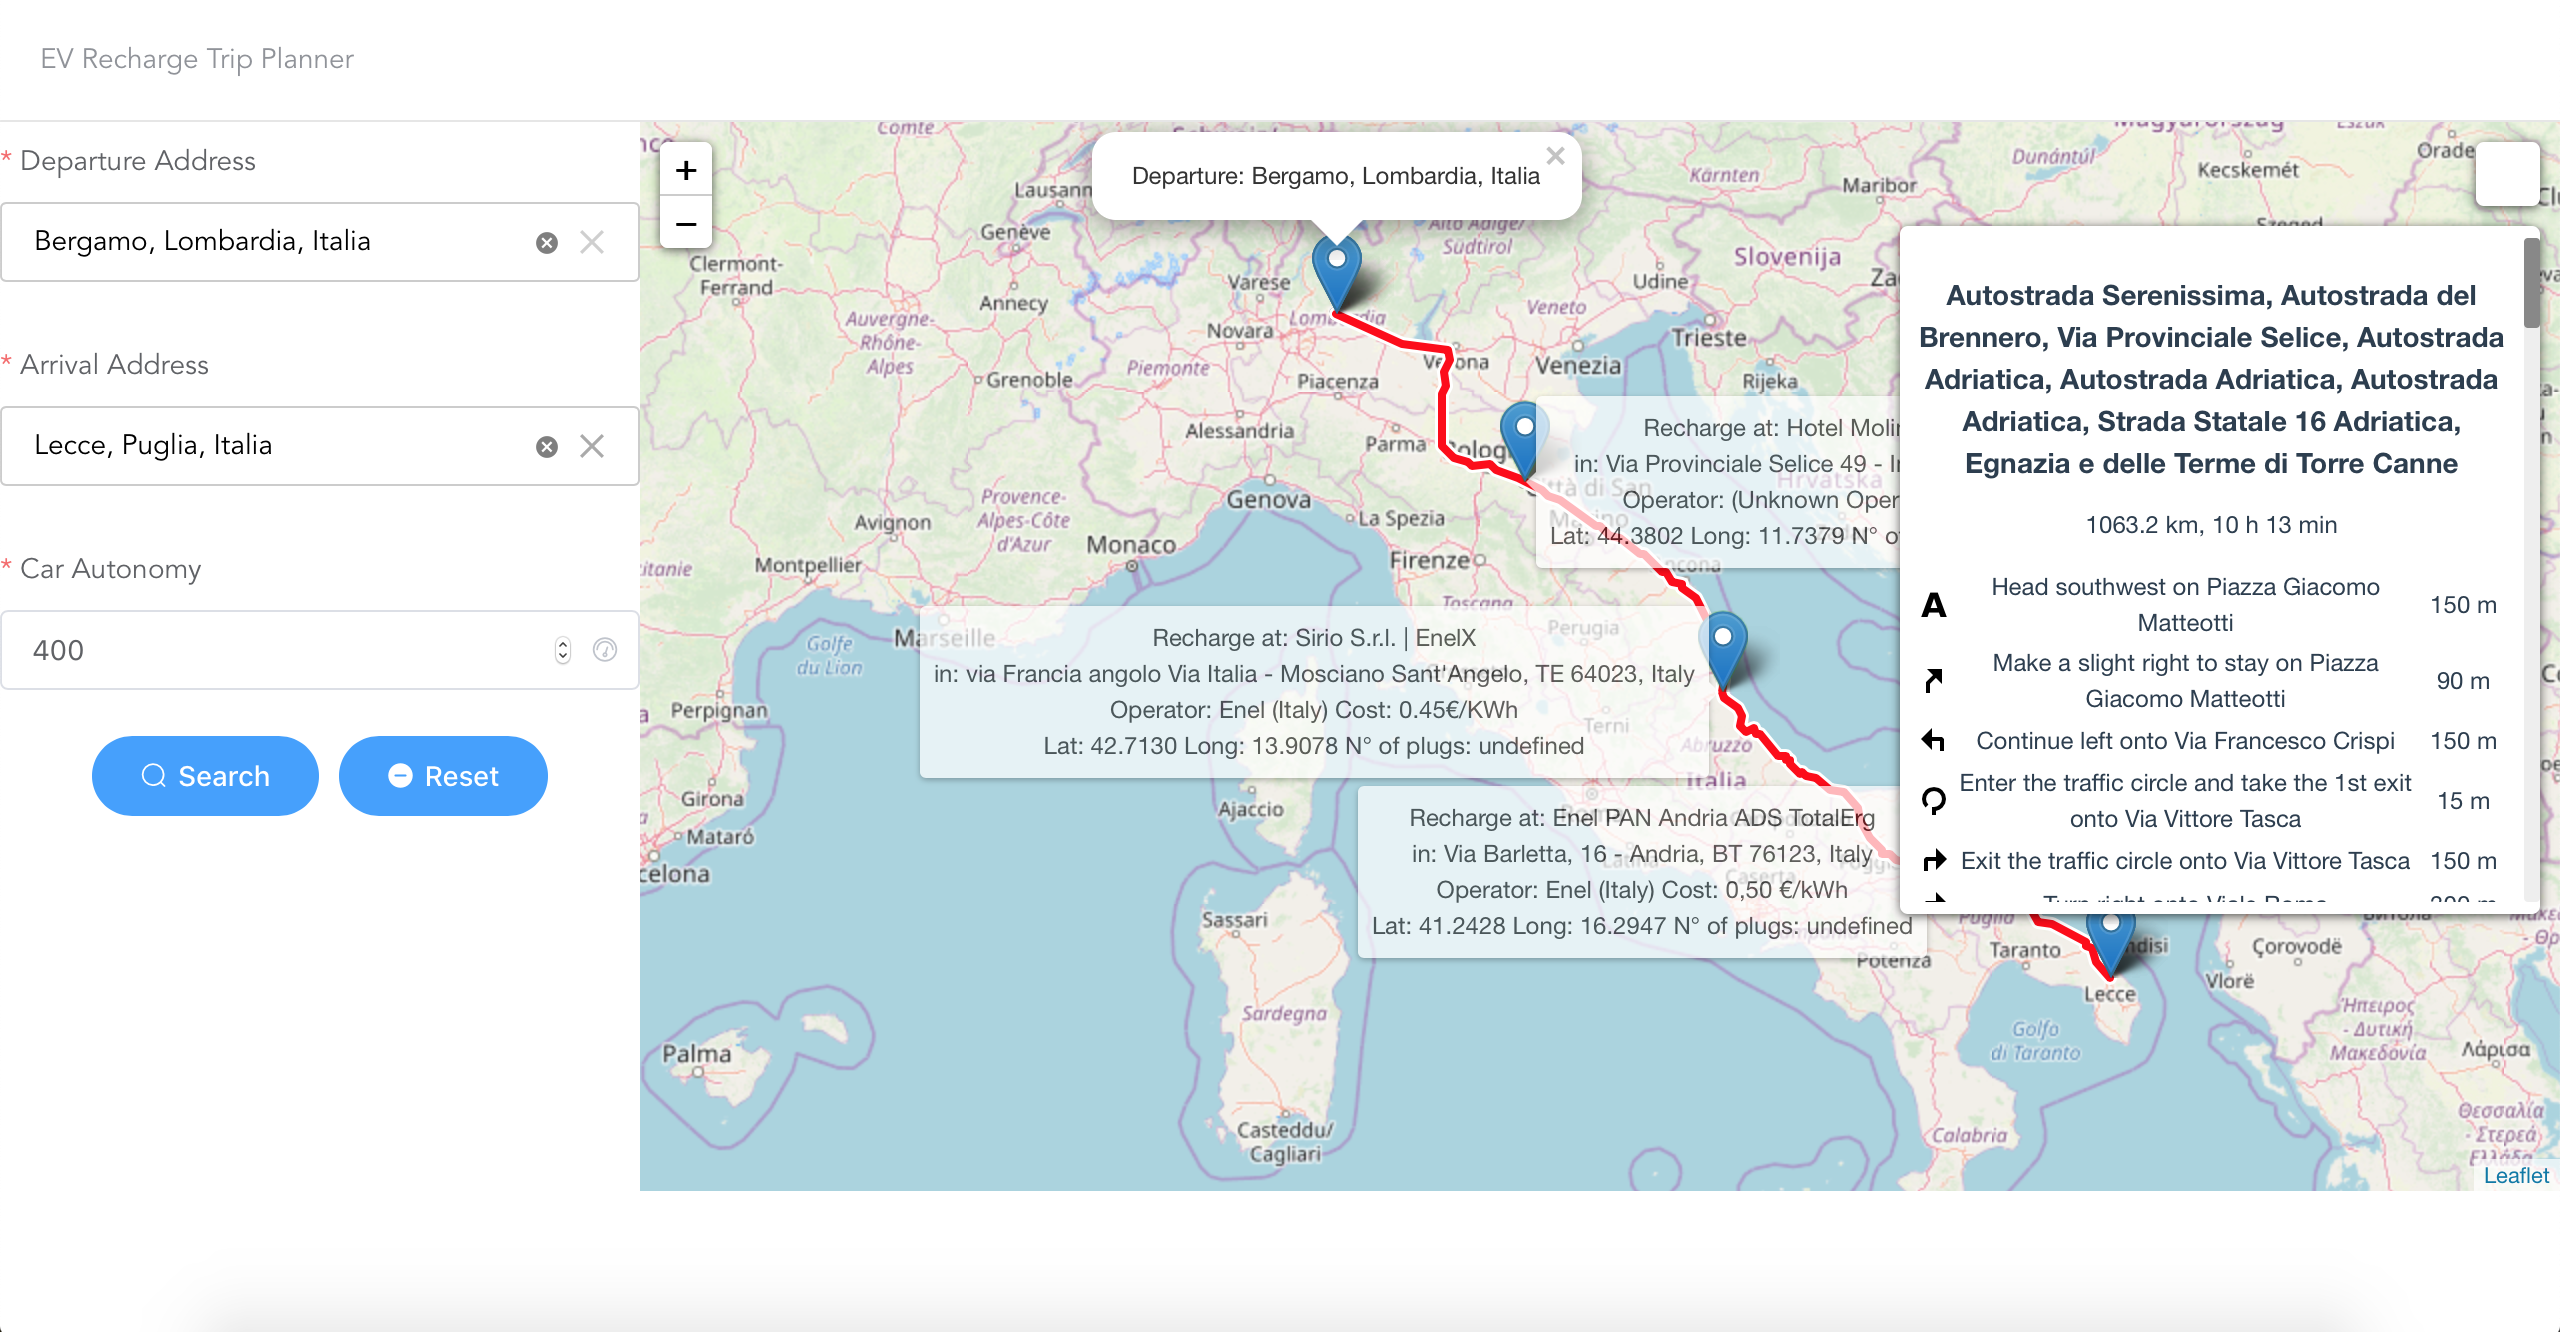
\includegraphics[scale=0.3]{Immagini/Schermata_esempio_planner.png}}
\caption{Schermata Esempio Planner 2}
\end{figure}

Una volta che l'utente ha visualizzato un determinato percorso esso potrà cancellare quello appena cercato ed effettuarne uno nuovo tramite il pulsante Reset come mostrato in Figura 10.7, la schermata che si presenterà è identica alla Homepage del programma.

\begin{figure}[h]
\centering
{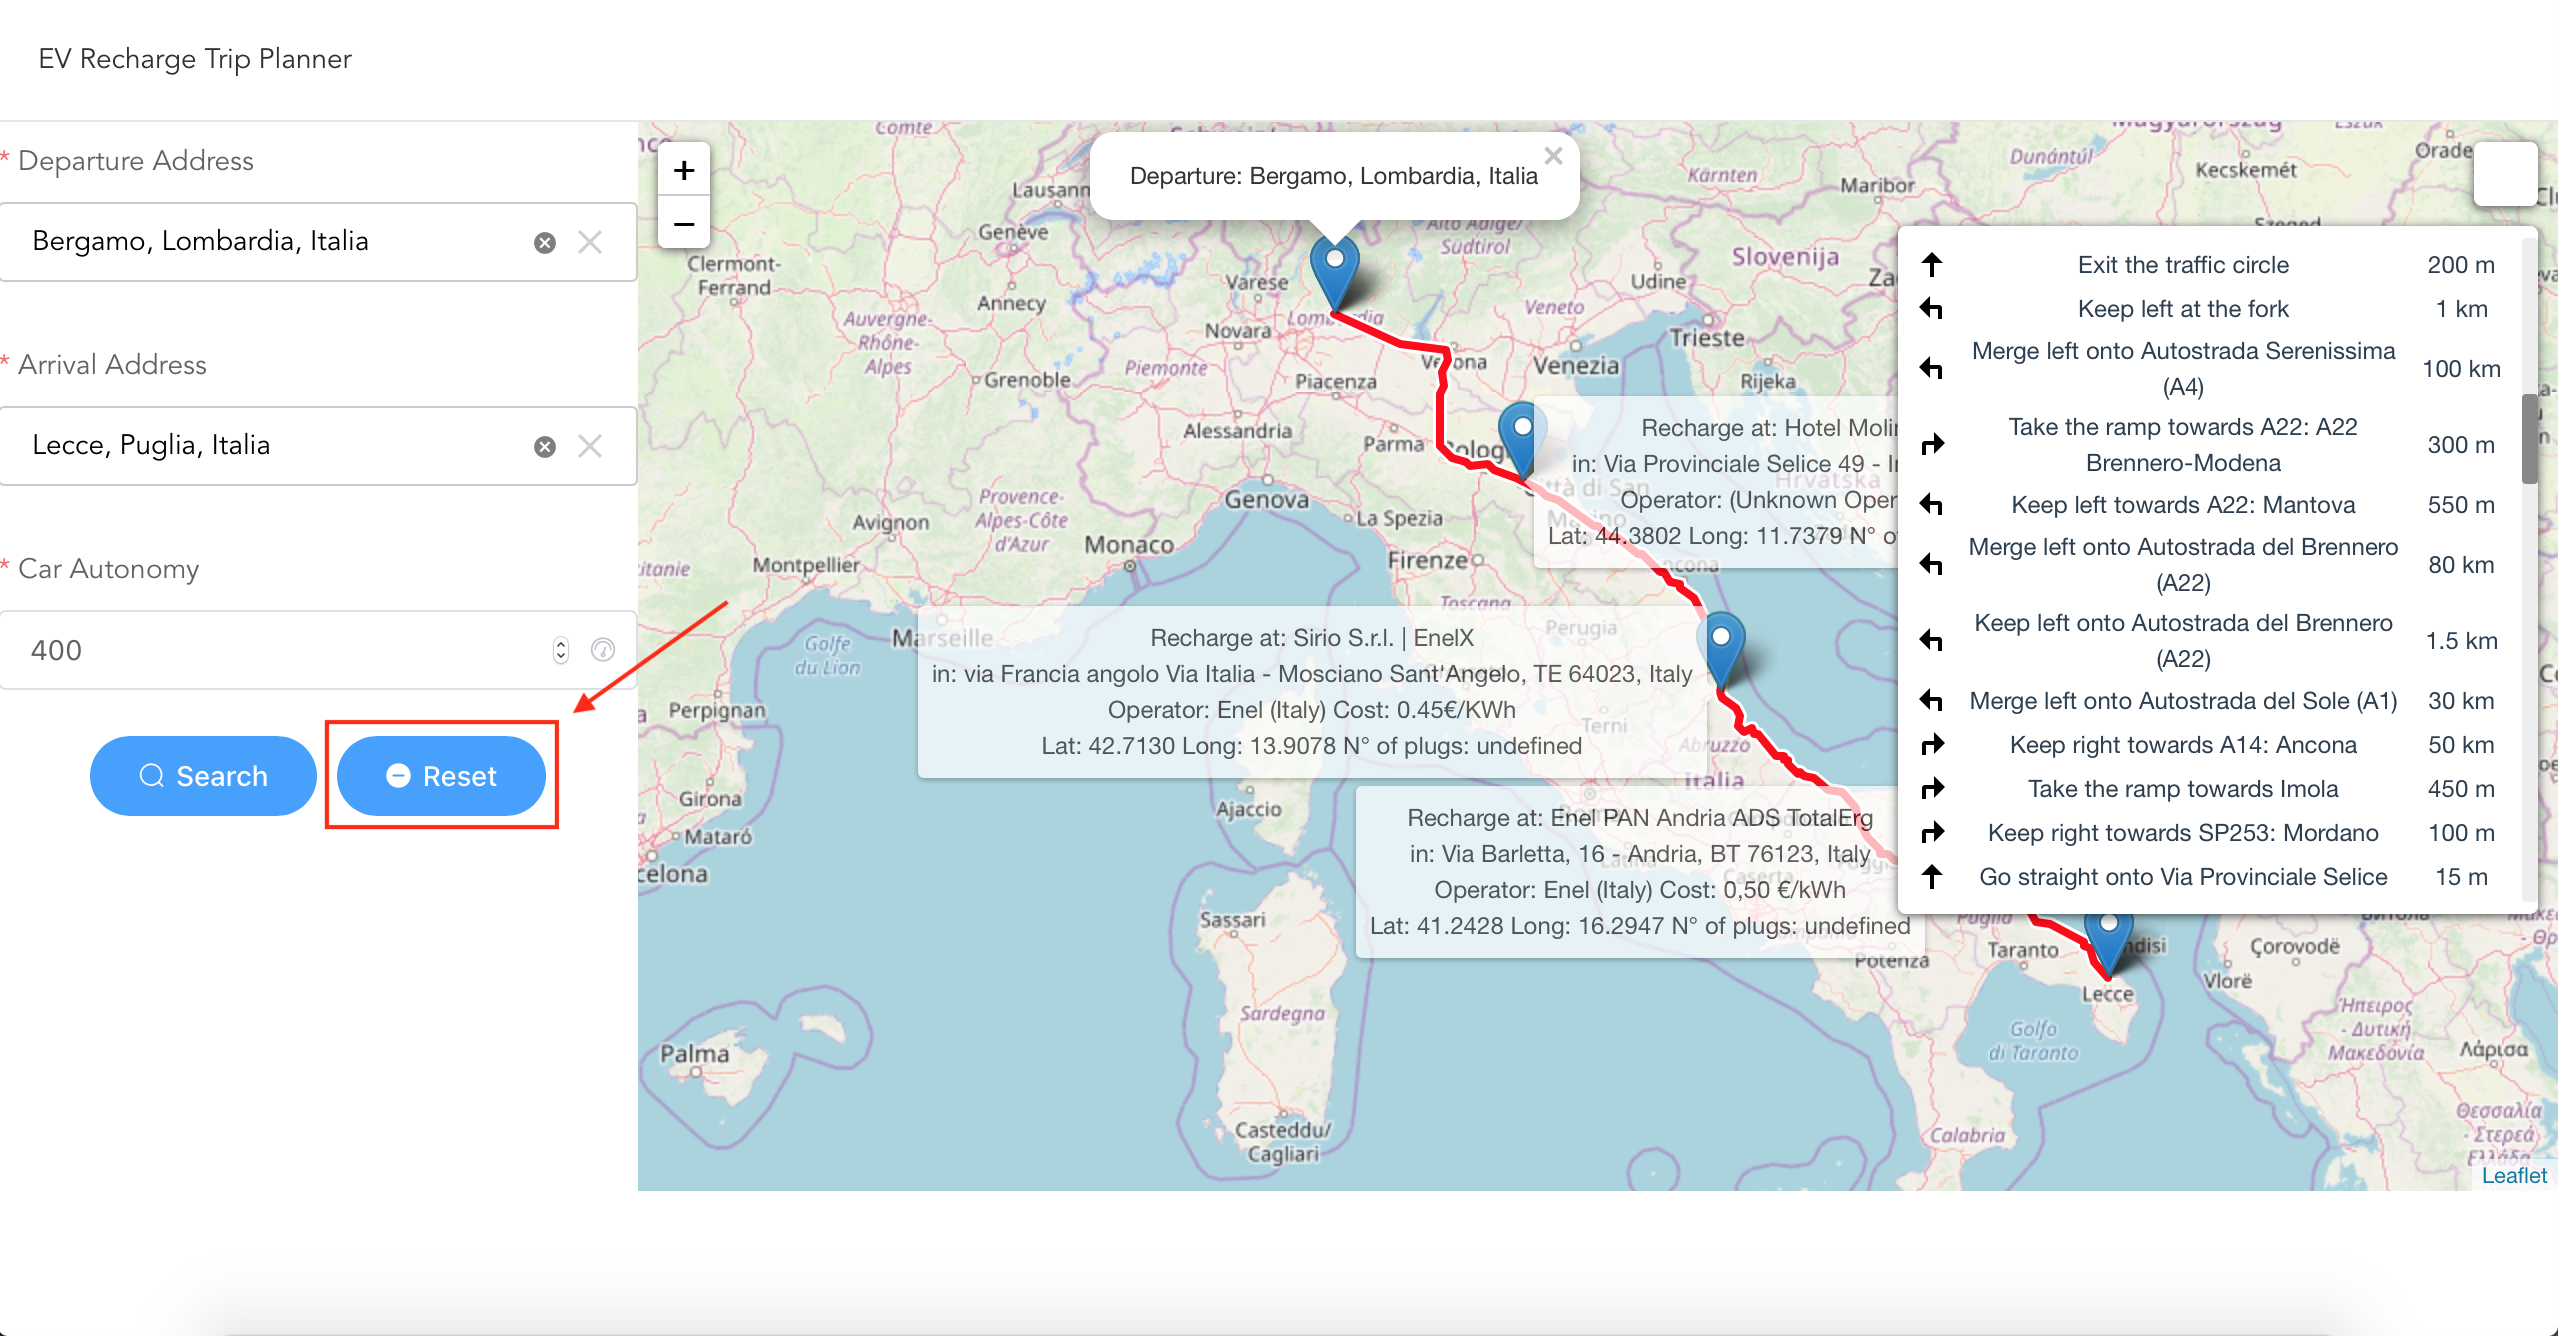
\includegraphics[scale=0.3]{Immagini/Schermata_esempio_planner_Reset.png}}
\caption{Schermata Esempio Planner 3}
\end{figure}




